\documentclass[11pt, oneside]{article}   	% use "amsart" instead of "article" for AMSLaTeX format
\usepackage{geometry}                		% See geometry.pdf to learn the layout options. There are lots.
\geometry{letterpaper}                   		% ... or a4paper or a5paper or ... 
%\geometry{landscape}                		% Activate for for rotated page geometry
%\usepackage[parfill]{parskip}    		% Activate to begin paragraphs with an empty line rather than an indent
\usepackage{graphicx}				% Use pdf, png, jpg, or eps� with pdflatex; use eps in DVI mode
								% TeX will automatically convert eps --> pdf in pdflatex		
\usepackage{amssymb}
\usepackage{amsmath}

\graphicspath{{/Users/telliott_admin/Dropbox/Tex/png/}}


\title{Formulas involving angle sum and difference}
%\author{The Author}
\date{}							% Activate to display a given date or no date

\graphicspath{{/Users/telliott_admin/Dropbox/Tex/png/}}

\begin{document}
\maketitle
%\section{}
%\subsection{}

\large
In this short write-up we'll look at the formulas for the sine and cosine of a sum of angles (and their difference, as well).  These formulas are used frequently in calculus to simplify expressions, and it would be very good to be familiar with them.  

To derive these expressions, start by considering the figure below.  In the left panel, we have a right triangle containing the angle $s$ at one vertex, and then draw above that a second right triangle with the angle $t$ at the same vertex, but rotated.   The two dotted lines are perpendicular to the base and the side of the first triangle, respectively.

Looking at the combined triangle with vertex angle $s+t$, the one that has the dotted vertical line as its side, we see that $s$ + $t$ + $u$ = 90 degrees.  Comparing with the rotated triangle containing  angle $t$ at the vertex, we see that the angle at the top of the figure (also labeled $s$) is actually equal to $s$ at the bottom left, because again $s$ + $t$ + $u$ = 90 degrees.

\begin{center}
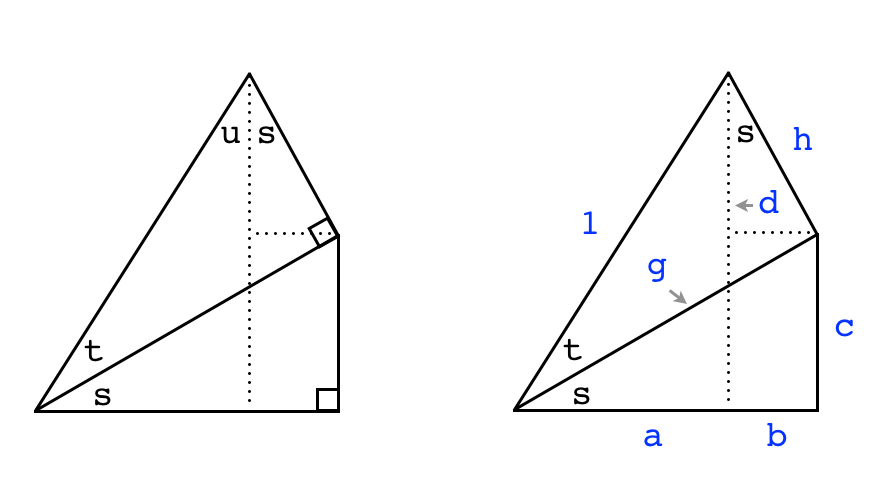
\includegraphics [scale=0.5] {sum_angle.png}
\end{center}

In the right panel, we label the sides for reference. The figure is scaled so that the hypotenuse of the upper triangle has length 1.  Now, we compute the sine and cosine of the angles $s$, $t$ and the sum of $s + t$: 

\[ cos \ s = \frac{a + b}{g},  \ \ \ \  cos \ t = g \]
\[ cos \ s \ cos \ t =  (\frac{a + b}{g}) \ g =  a + b \]
\[ cos(s+t) = a =  a + b - b  = cos \ s \ cos \ t - b \]
We need to find an expression for $b$.  From angle $s$ at the top of the figure  
\[ sin \ s = \frac{b}{h}, \ \ \ \  sin \ t = h, \ \ \ \  sin \ s \ sin \ t = \frac{b}{h} h = b \]
\[ cos(s+t) = cos \ s \ cos \ t - b \]

\begin{equation}
 \boxed{ cos(s+t) = cos \ s \ cos \ t - sin \ s \ sin \ t}
\end{equation}

\subsection*{difference}

The formula for the cosine of the difference of angles ($s-t$) is the same, but the second term becomes positive in sign.  This can be seen by substituting $-t$ for $t$.  Then

\[ sin \ t = -sin(-t), \ \ \ \ cos \ t = cos(-t)\]
We have
\[ cos(s-t) = cos \ s \ cos(-t) - sin \ s \ sin(-t) \]
\[ = cos \ s \ cos \ t + sin \ s \ sin \ t \]
Notice that this checks for $s=t$
\[ cos(s-t) = cos \ s \ cos \ t + sin \ s \ sin \ t \]
\[ cos(0) = 1 = cos^2 \ s \ + sin^2 \ s \]

\subsection*{sine($s+t$)}

One can use the same geometric construction (using the two segments of the height) to derive the formulas for the sum and difference of sine.  Let's look at the figure again

\begin{center}
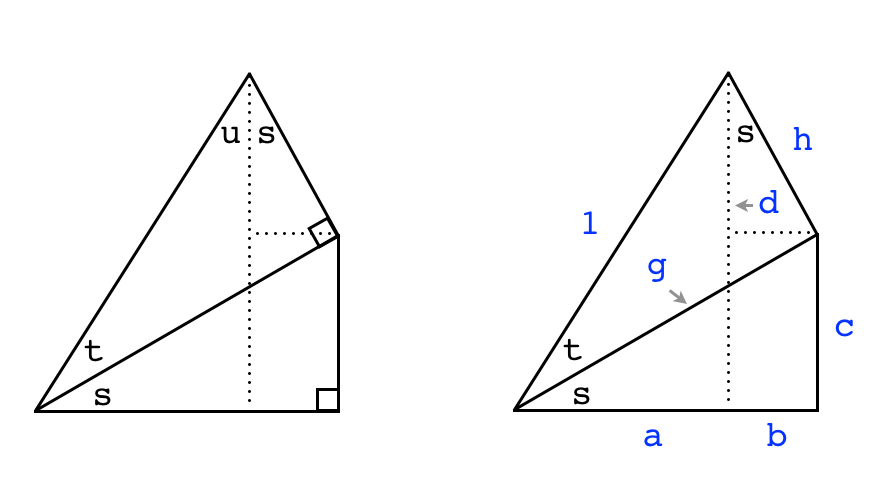
\includegraphics [scale=0.5] {sum_angle.png}
\end{center}

\[ sin(s+t) = c + d \]
\[ sin \ s = \frac{c}{g} \]
\[cos \ t = g \]
\[ sin \ s \ cos \ t = c \]
\[ sin(s+t) =  sin \ s \ cos \ t  + d \]
We need an expression for $d$.  Looking at the small top triangle:
\[ cos \ s = \frac{d}{h} \]
\[ sin \  t = h \]
\[ d = sin \ t \ cos \  s \]
\[ sin(s+t) =  sin \ s \ cos \ t  + sin \ t + cos \ s  \]

\subsection*{another way}

There is a different way that's perhaps quicker. (Although I have to confess that I always find this part confusing).  

Recall that
\[ cos ( \theta + \frac{\pi}{2})= -sin \ \theta \]
This is a fundamental identity in trigonometry, and it's worth pointing out that it is consistent with the sum of cosines formula above  
\[ cos(s+t) = cos \ s \ cos \ t - sin \ s \ sin \ t \]
\[ cos(s+\frac{\pi}{2}) = cos \ s \ cos \ \frac{\pi}{2} - sin \ s \ sin \ \frac{\pi}{2} \]
\[ cos(s+\frac{\pi}{2}) = cos \ s \times 0 - sin \ s \times 1 \]
\[ cos(s+\frac{\pi}{2}) = - sin \ s \]
Also
\[ sin ( \theta + \frac{\pi}{2})= cos \ \theta \]
Substitute $s+t$ for $\theta$ into the above
\[ cos ( \theta + \frac{\pi}{2})= -sin \ \theta \]
\[ cos ( s + t + \frac{\pi}{2})= -sin (s + t) \]
We have part of what we want:  $sin(s+t)$!  Now, simply by grouping the terms on the left-hand side in another way we obtain
\[ cos(s + t + \frac{\pi}{2}) \]
\[ cos(s + (t + \frac{\pi}{2})) \]
Using the formula for sum of cosines this is
\[ cos(s + (t + \frac{\pi}{2})) = cos \ s \ cos (t + \frac{\pi}{2}) - sin \ s \ sin(t + \frac{\pi}{2}) \]
Now consider the term on the right-hand side containing
\[ \ cos (t + \frac{\pi}{2}) \]
Reverse the substitution using the first identity
\[ cos ( t + \frac{\pi}{2})= -sin \ t \]
\[ cos \ s \ cos (t + \frac{\pi}{2}) = cos \ s \ (-sin \ t) \]
Similarly, for the term
\[ sin(t + \frac{\pi}{2}) \]
Reverse the substitution using
\[ sin(t + \frac{\pi}{2}) = cos \ t \]
\[ sin \ s \ sin(t + \frac{\pi}{2}) = sin \ s \ cos \ t \]
So putting it all together 
\[ -sin (s + t) = cos \ s \ (-sin \ t) - sin \ s \ cos \ t \]
Finally, multiply by each term by $-1$
\begin{equation}
 \boxed{ sin (s + t) = cos \ s \ sin \ t + sin \ s \ cos \ t}
\end{equation}

\subsection*{difference}

As before, the difference is the same but with the sign of the second term switched, using the same simple trick as before.
\[sin(s-t) = sin\ s\ cos\ t\ - sin\ t\ cos\ s\]
These formulas are so useful that you should try to memorize at least one of them.  But I picked only one to remember, that one is 
\[ cos(s-t) = cos \ s \ cos \ t + sin \ s \ sin \ t \]
That's because it's easily checked by setting s = t, as we saw above.

The other formulas can be generated from this one because they are different.  The sine formulas involve products of sine and cosine, and the sign of the second term is opposite.

\subsection*{Euler}

However, the way I really remember these (as a fallback if I've forgotten, which happens) is to use Euler's famous formula:
\begin{equation}
 \boxed{ e^{i \theta} = cos \ \theta + i \ sin \ \theta}
\end{equation}
Substitute $\theta=s+t$
\[  e^{i (s+t)} = cos (s+t) + i \ sin (s+t)        \]
but
\[  e^{i (s+t)} = e^{is} e^{it} \]
\[ e^{i (s+t)} = (cos \ s + i \ sin \ s)  (cos \ t + i \ sin \ t)        \]
\[ cos (s+t) + i \ sin (s+t) = (cos \ s + i \ sin \ s)  (cos \ t + i \ sin \ t)        \]
For these last two to be equal, both the real and the imaginary parts must be equal.  Multiplication leads directly to the correct formulas.  For example, the real part is
\[ \cos(s+t) = cos \ s \ cos \ t + i^2 sin \ s \ sin \ t = cos \ s \ cos \ t - sin \ s \ sin \ t \]
That is remarkably easy, and complete.

\subsection*{double- and half-angle}

As long as we're at it, we might as well add the so-called half-angle and double-angle formulas.  For the double-angle, from above we have
\[ cos(s+t) = cos \ s \ cos \ t - sin \ s \ sin \ t \]
If $s=t$ we have
\[ cos(2s) = cos^2(s) - sin^2(s)  = 2 \ cos^2(s) - 1\]
\[cos^2(s) = \frac{1}{2} [1 + cos(2s)] \]
And
\[sin(s+t) = sin\ s\ cos\ t\ + sin\ t\ cos\ s\]
If $s=t$ we have
\[sin(2s) = 2 \ sin\ s\ cos\ s \]
Converting from the double-angle to the half-angle (with $u = 2s$)
\[cos^2(\frac{u}{2}) = \frac{1}{2} [1 + cos(u)] \]
\[sin(u) = 2 \ sin\ \frac{u}{2} \ cos\  \frac{u}{2} \]
These are dummy variables (we could pick any letters), so the formulas can be written with $x$ or $s$ or $\theta$, as you please.

\subsection*{another approach}
In a different write-up, we derived the matrix for rotation of a vector 

\[
\begin{bmatrix}   
\cos \theta & -\sin \theta  \\  \sin \theta &\ \  \cos \theta  \end{bmatrix}
\begin{bmatrix}   x   \\  y  \end{bmatrix} = \begin{bmatrix}   u   \\  v  \end{bmatrix}
\]
We can think of rotation by the angle $s+t$ as the sequential application of this matrix, first for the angle $s$ and then for the angle $t$.  That is
\[
\begin{bmatrix}   
\cos s+t & -\sin s+t  \\ 
\sin s+t &\ \  \cos s+t  
\end{bmatrix}
=
\begin{bmatrix}   
\cos s & -\sin s  \\ 
\sin s &\ \  \cos s  
\end{bmatrix}
\begin{bmatrix}   
\cos t & -\sin t  \\ 
\sin t &\ \  \cos t  
\end{bmatrix}
\]
By the rules of matrix multiplication, the upper left entry of the product is:
\[ \cos \ s+t =  \cos \ s \  \cos \ t - \sin \ s \ \sin \ t  \]
and the lower left entry is
\[ \sin \ s+t =  \sin \ s \  \cos \ t + \cos \ s \ \sin \ t  \]
Pretty neat!


\end{document}  